\section{Porte}
Sur l'image ci-dessous, la porte dans son état original :
\begin{figure}[H]
    \centering
    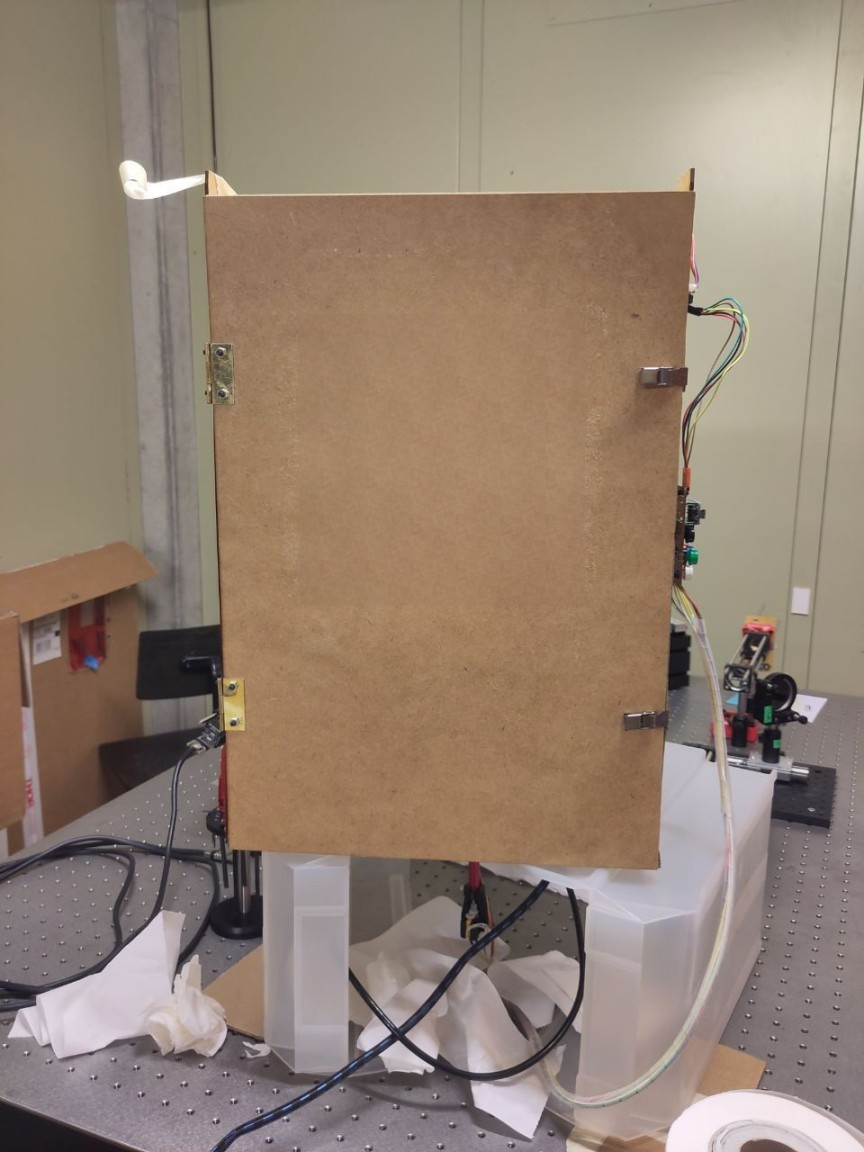
\includegraphics[width=0.5\textwidth]{assets/figures/ameliorations/porte_sans_fenetre.png}
    \caption{Photo de la porte avant modification}\label{photo porte}
\end{figure}

\newpage
Après une découpe dans le panneau de la porte, et le design de pièces de fixations et d'un chablon de perçage,
la porte est désormais équipée d'une fenetre:
\begin{figure}[H]
    \centering
    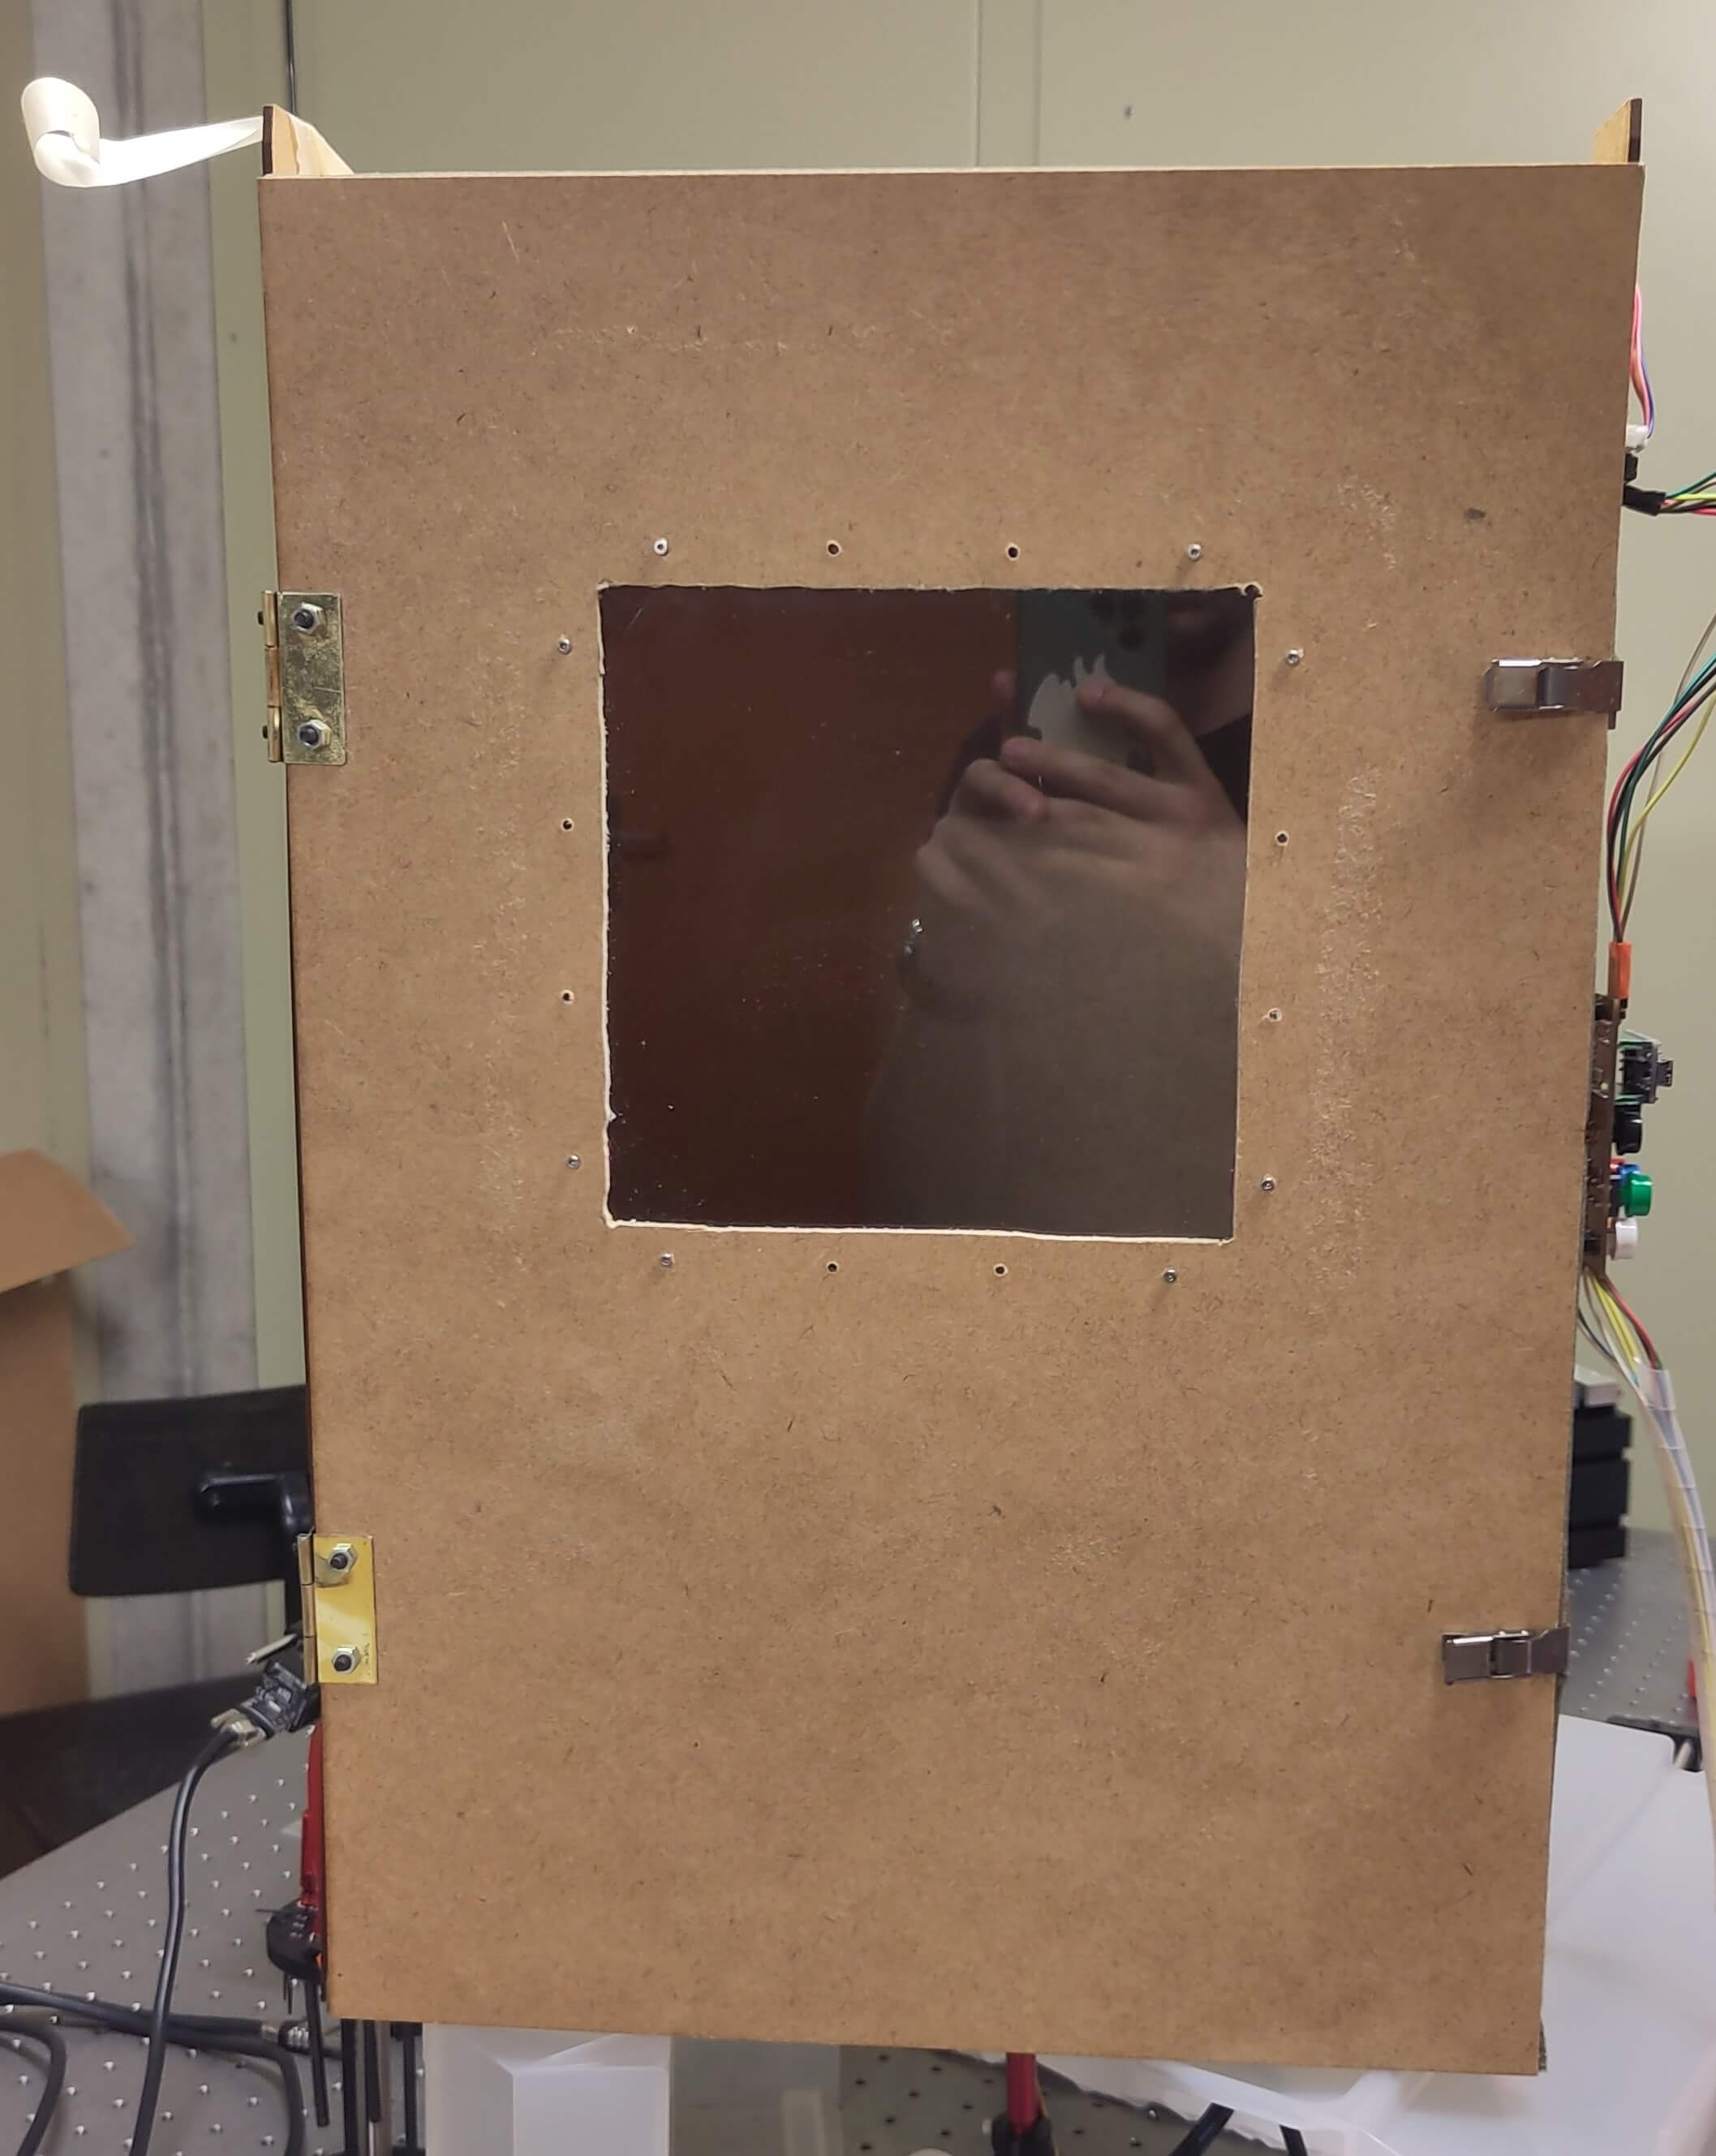
\includegraphics[width=0.5\textwidth]{assets/figures/ameliorations/porte_avec_fenetre.jpg}
    \caption{Photo de la porte après modification}\label{photo porte fenetre}
\end{figure}

DECRIRE FIXATION


\newpage
\section{Mesures}
\subsection{Problématique et situation d'origine}
Le procédé de mesure d'origine est sommaire et nécessite beaucoup de temps, en effet il convient de:
\begin{enumerate}
    \item Placer le disque dans le faisceau :
          \begin{figure}[H]
              \centering
              
\includegraphics[width=0.5\textwidth]{assets/figures/Placeholder.jpeg}
              \caption{Placeholder}\label{Placeholder}
          \end{figure}

    \item Attendre quelques secondes que la mesure sur le logiciel soit stable:
          \begin{figure}[H]
              \centering
              
\includegraphics[width=0.5\textwidth]{assets/figures/Placeholder.jpeg}
              \caption{Placeholder}\label{Placeholder}
          \end{figure}

    \item Prendre la mesure l'enregistrer en format \textbf{.csv} avec le numéro de mesure.
    \item Tourner le disque d'un petit angle:
          \begin{figure}[H]
              \centering
              
\includegraphics[width=0.5\textwidth]{assets/figures/Placeholder.jpeg}
              \caption{Placeholder}\label{Placeholder}
          \end{figure}
\end{enumerate}

Répéter en suite les étapes \textbf{2 à 4} pour autant de mesures qu'il le faut.
Dans le cadre de ce projet, plus il y a de données mieux c'est, il convient donc d'automatiser le
processus de prise de mesure au maximum pour pouvoir caractériser les écrans de turbulance facilement.

